\documentclass[tikz,border=10pt]{standalone}
\usetikzlibrary{angles}
\begin{document}
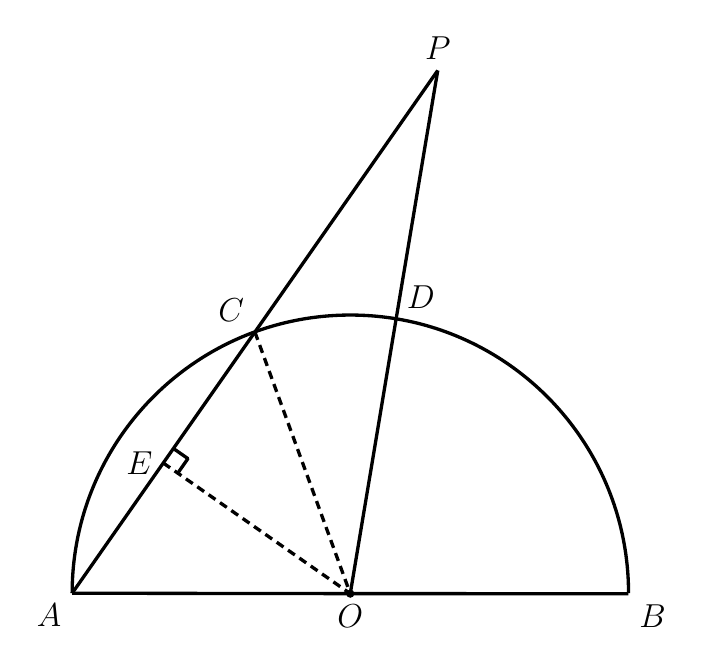
\begin{tikzpicture}[line width=1.2pt, line join=round]
\coordinate (A) at (-3.555,-3.305);
\coordinate (B) at (3.510,-3.311);
\coordinate (C) at (-1.234,0.012);
\coordinate (D) at (0.559,0.177);
\coordinate (O) at (-0.023,-3.310);
\coordinate (P) at (1.088,3.334);
\coordinate (GeoTailC) at (1.019,3.236);











\coordinate (E) at (-2.398,-1.651);


\draw[solid] (A) -- (O) -- (B);
\fill (O) circle (1.500pt);


\draw (A) arc[start angle=180.000, end angle=0.000, radius=3.533];


\draw[solid] (A) -- (E) -- (C) -- (GeoTailC) -- (P);


\draw[solid] (P) -- (D) -- (O);


\draw[dash pattern=on 3pt off 2pt] (E) -- (O);
\draw[dash pattern=on 3pt off 2pt] (C) -- (O);


\draw pic[draw, angle radius=0.225cm] {right angle=P--E--O};


\node[below left, font=\fontsize{12}{14.4}\selectfont] at (A) {$A$};
\node[below, font=\fontsize{12}{14.4}\selectfont] at (O) {$O$};
\node[below right, font=\fontsize{12}{14.4}\selectfont] at (B) {$B$};
\node[above, font=\fontsize{12}{14.4}\selectfont] at (P) {$P$};
\node[above left, font=\fontsize{12}{14.4}\selectfont] at (C) {$C$};
\node[above right, font=\fontsize{12}{14.4}\selectfont] at (D) {$D$};
\node[left, font=\fontsize{12}{14.4}\selectfont] at (E) {$E$};
\end{tikzpicture}
\end{document}